\documentclass[11pt,a4paper]{article}
\usepackage[latin5]{inputenc}
\usepackage[english]{babel}
\usepackage{amsmath}
\usepackage{amsfonts}
\usepackage{amssymb}
\usepackage{graphicx,subfig}
\usepackage{placeins}
\usepackage{gensymb}

\author{Alexander Attinger, Yannic Kilcher}
\title{Report Blatt 7, Advanced Part}

\begin{document}
\maketitle

\section{3D Reconstruction}

We built up a pipeline to do image reconstruction where we first preprocess two stereo images. After that we use the kown algorithms from the previous exercises to find feature points and match them. From the best matches we calculate the fundamental matrix and rectify our processed images. From this, we can calculate a depth map, which we try to visualize with the point cloud library. The results can be seen in Fig. \ref{fig:e1}.

\begin{figure}%
\centering
\subfloat[][Original Image]{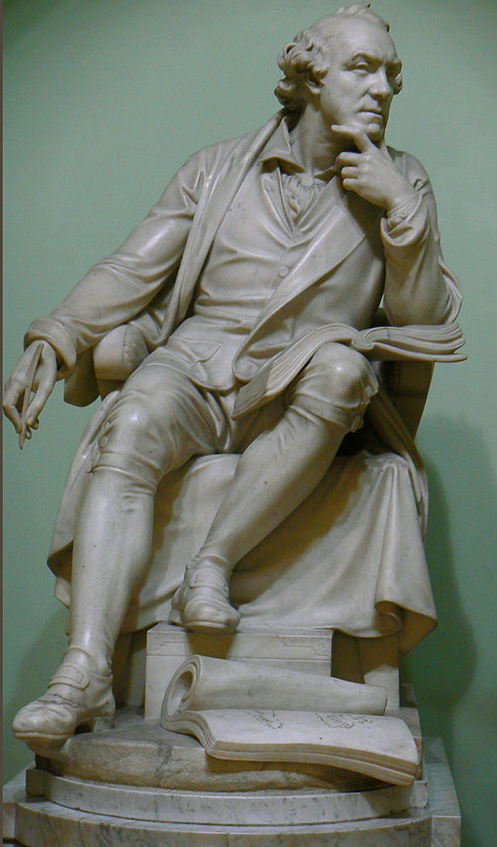
\includegraphics[scale=.2]{data/johnHunter/001.png}}
\quad
\subfloat[][Good SURF matches]{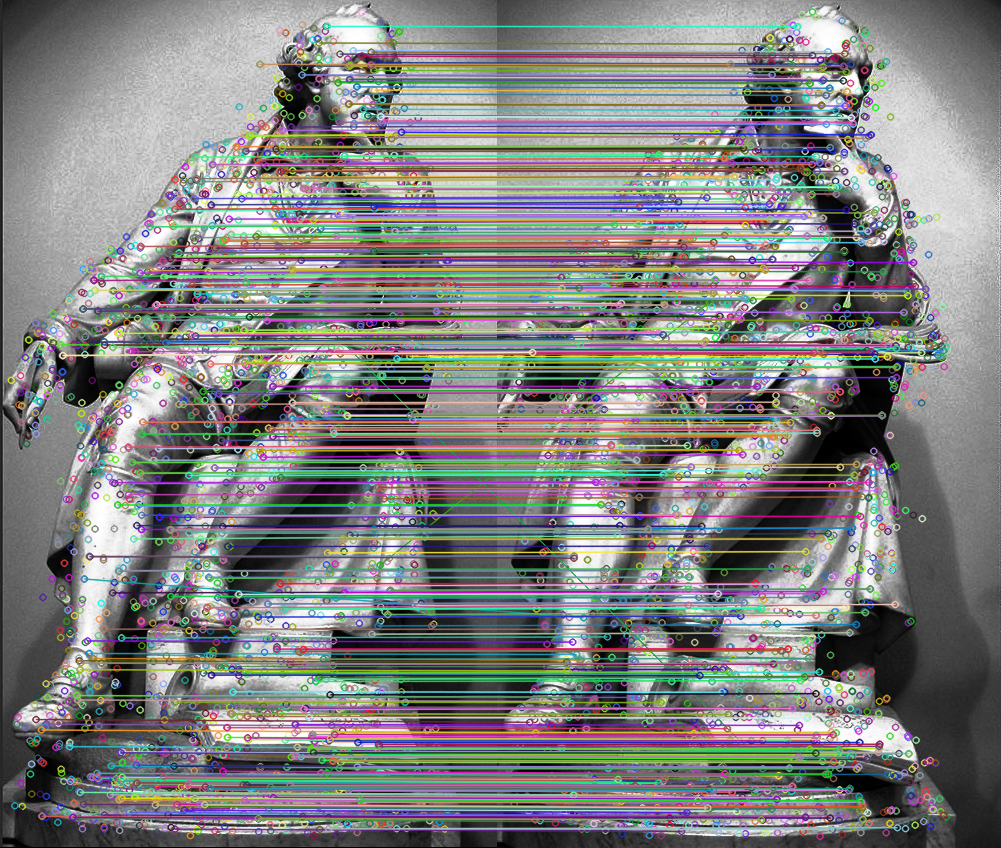
\includegraphics[scale=.2]{data/res/Matches_surf_02.png}}
\quad
\subfloat[][Example dispairity map]{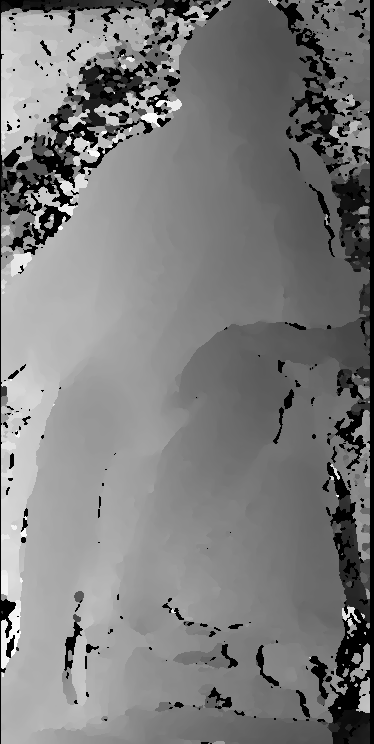
\includegraphics[scale=.2]{data/res/dispmapjh.png}}
\quad
\subfloat[][Side view of the 3D reconstruction (looks better when you're able to play with it)]{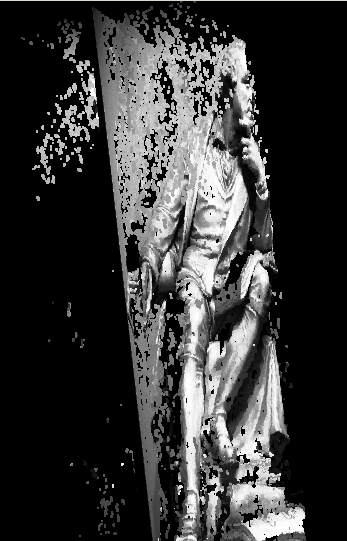
\includegraphics[scale=.2]{data/res/johnhunter1.png}}
\quad
\caption{3D reconstruction of John Hunter using our own pipeline}%
\label{fig:e1}%
\end{figure}

\section{Optical Flow}

By using OpenCV's built-in functions, we calculate the optical flow between two stereo images. Through observing, which points move further than others, we can estimate a depth map. Again we use this to visualize the images via the point cloud libraries. Unfortunately, our OpenCV distribution did not include color maps, so we could only do greyscale visualizations of stuff. The results can be seen in Figures \ref{fig:e2} and \ref{fig:e3}.

\begin{figure}%
\centering
\subfloat[][Original Image]{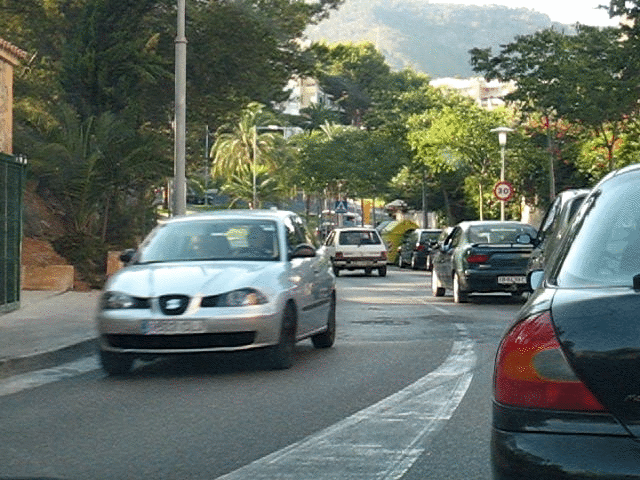
\includegraphics[scale=.2]{data/car/input1.png}}
\quad
\subfloat[][Grayscale visualization of the optical flow's direction]{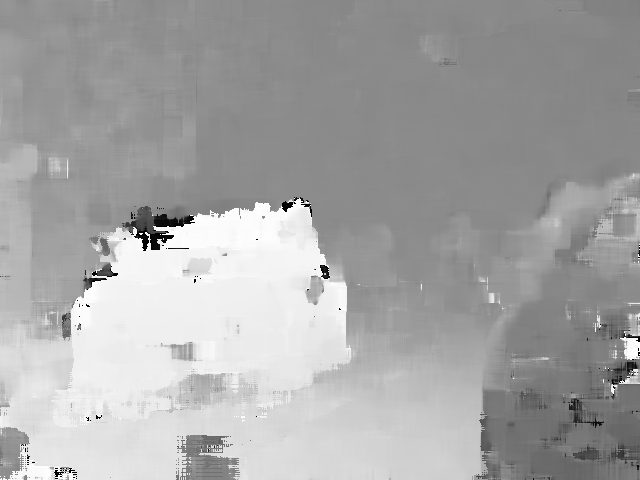
\includegraphics[scale=.2]{data/res/optical_flow_direction_car.png}}
\quad
\subfloat[][Grayscale visualization of the optical flow's magnitude (used as depth map)]{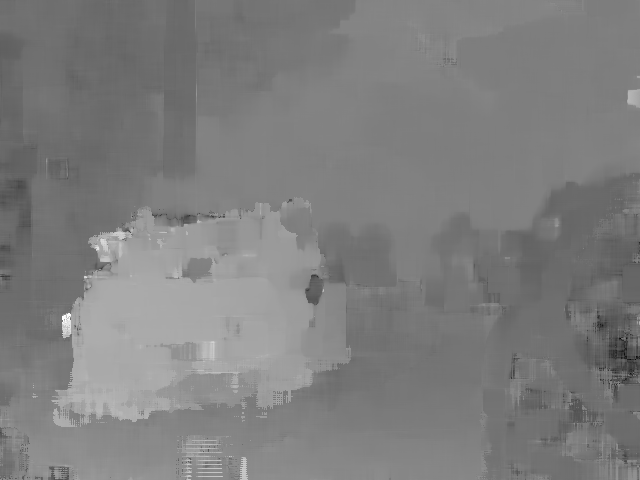
\includegraphics[scale=.2]{data/res/optical_flow_norm_car.png}}
\quad
\subfloat[][Final Reconstruction]{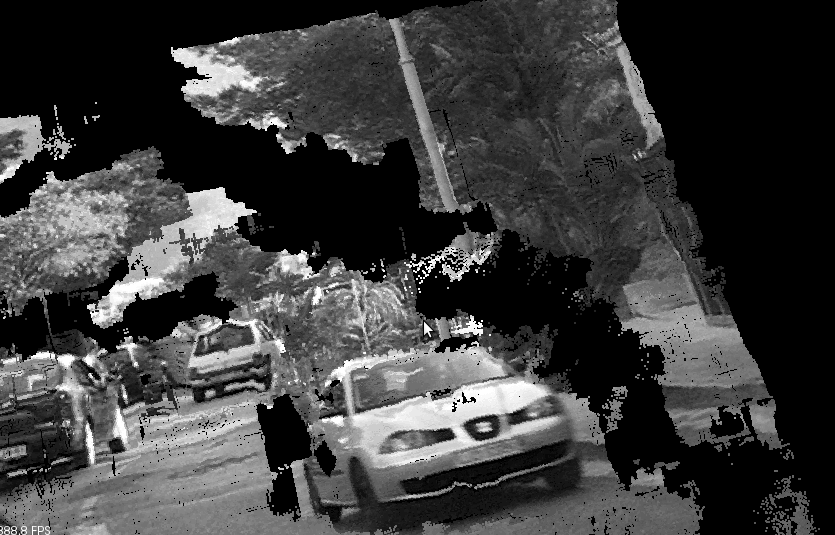
\includegraphics[scale=.2]{data/res/ddcar.png}}
\quad
\caption{3D reconstruction of a car using optical flow}%
\label{fig:e2}%
\end{figure}

\begin{figure}%
\centering
\subfloat[][Original Image]{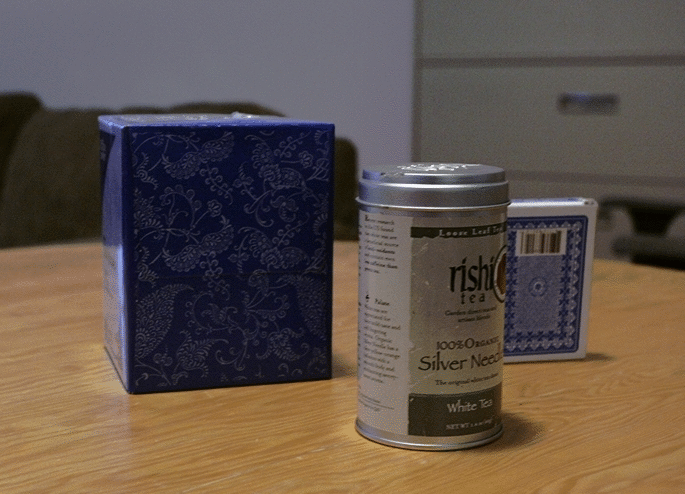
\includegraphics[scale=.2]{data/table/input1.png}}
\quad
\subfloat[][Grayscale visualization of the optical flow's direction]{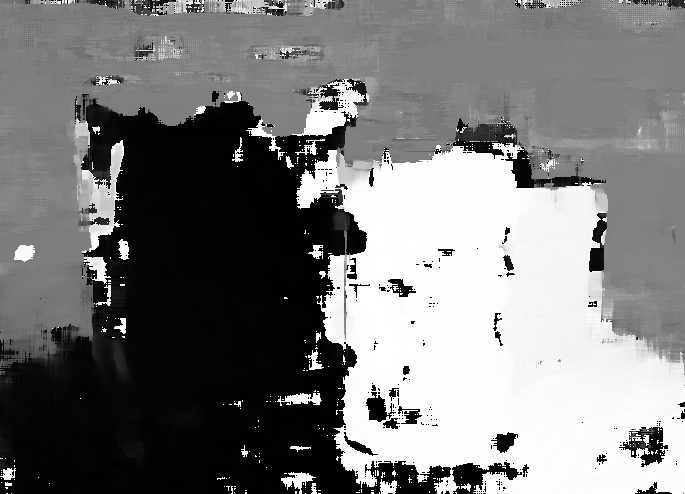
\includegraphics[scale=.2]{data/res/optical_flow_direction_table.png}}
\quad
\subfloat[][Grayscale visualization of the optical flow's magnitude (used as depth map)]{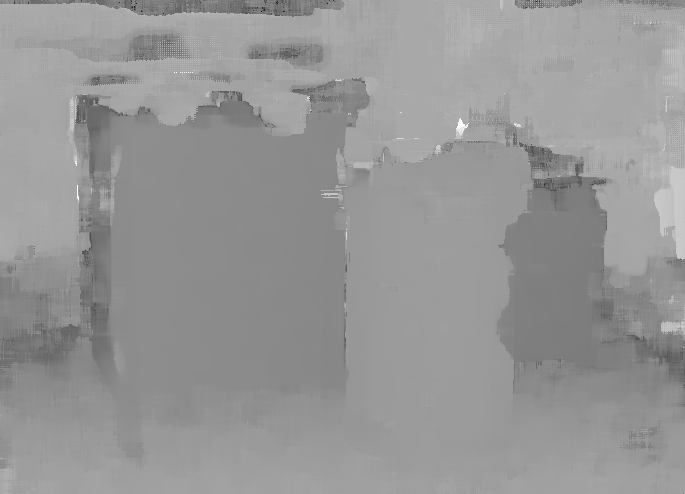
\includegraphics[scale=.2]{data/res/optical_flow_norm_table.png}}
\quad
\subfloat[][Final Reconstruction]{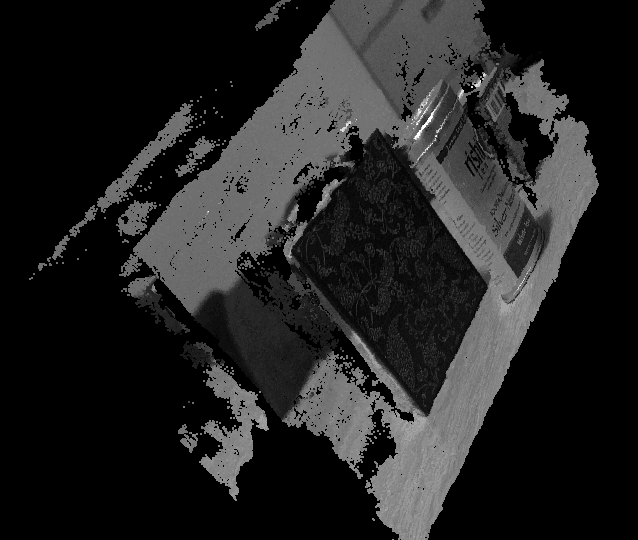
\includegraphics[scale=.2]{data/res/ddtbl.png}}
\quad
\caption{3D reconstruction of a table using optical flow}%
\label{fig:e3}%
\end{figure}

\section*{Conclusion}
In conclusion, this exercise was the most time consuming. Not too much the programming part, as the getting all the libraries in place and getting it to run correctly, as well as constantly converting between numerous formats so that the different libraries could take our data as parameters. In the end, the 3D reconstructions didn't work out quite as well as we'd hoped, but at least we got an idea how to go about such a task.
Also it was difficult to get the scaling right, especially going from the optical flow magnitude to the depth map, we had to apply some nonlinear transformations (roots, logs), otherwise, a handful of points would have stood out really far from the picture and all the others would have been flat. The paramter tuning is critical to the success of these exercises and we are convinced that, given more time, we could get better results by simply finding the right values.

\end{document}
